\scanpage{65}
% archive sheet number: 64
% @ upper left, date
3.1.84

% @ upper left, first surface
\figure{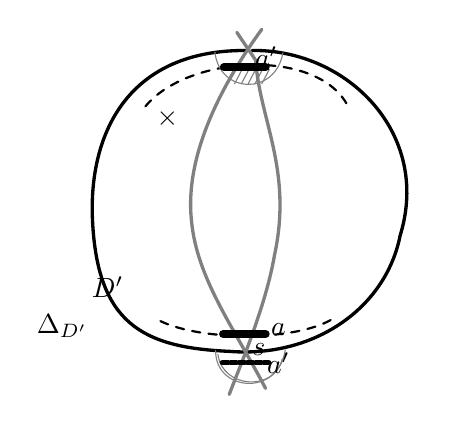
\begin{tikzpicture}[x=.96cm,y=.96cm,line cap=round,line join=round]
\draw[very thick] (0,2) .. controls (-1.52,2.01) and (-2.08,.95) .. (-2.03,-.23) .. controls (-1.97,-1.6) and (-1.38,-1.93) .. (-.22,-1.98) .. controls (.9,-2.07) and (1.85,-1.41) .. (2.04,-.45) .. controls (2.46,.91) and (1.33,2.02) .. (.08,2);
\draw[very thick,gray] (.21,2.28) .. controls (-.24,1.66) and (-.82,.68) .. (-.72,-.25) .. controls (-.65,-1.02) and (-.15,-1.68) .. (.26,-2.47);
\draw[very thick,gray] (-.12,2.24)--(.13,1.87) .. controls (.18,1.09) and (.62,.42) .. (.38,-.7) .. controls (.26,-1.4) and (-.09,-2.2) .. (-.22,-2.55);
\draw[thick,dashed] (-1.33,1.26) .. controls (-.78,1.93) and (.9,2.04) .. (1.33,1.3);
\draw[thick,dashed] (-1.13,-1.58) .. controls (-.57,-1.85) and (.71,-1.85) .. (1.18,-1.53);
\draw[gray] (-.41,1.98) .. controls (-.35,1.42) and (.39,1.4) .. (.49,1.97);
\draw[gray] (-.4,-1.97) .. controls (-.41,-2.51) and (.43,-2.59) .. (.52,-1.96);
\draw[gray] (-.37,-2.02) .. controls (-.31,-2.48) and (.39,-2.51) .. (.48,-2.08);
\foreach \x in {-.24,-.15,-.06,.03,.12,.21}{\draw[thin,gray] (\x,1.56)--++(.10,.19);}
\draw[line width=3pt] (-.29,1.78)--(.26,1.78) (-.30,-1.75)--(.26,-1.75);
\draw[line width=2pt,densely dotted] (-.31,-2.13)--(.30,-2.13);
\node at (-1.04,1.10) {$\times$};\node at (.27,1.91) {$a'$};
\node at (.43,-1.69) {$a$};\node at (.43,-2.13) {$a'$};\node at (.17,-1.95) {$s$};
\node at (-1.83,-1.13) {$D'$};\node at (-2.43,-1.65) {$\Delta_{D'}$};
\end{tikzpicture}\hspace{.55em}
% @ upper centre, second surface
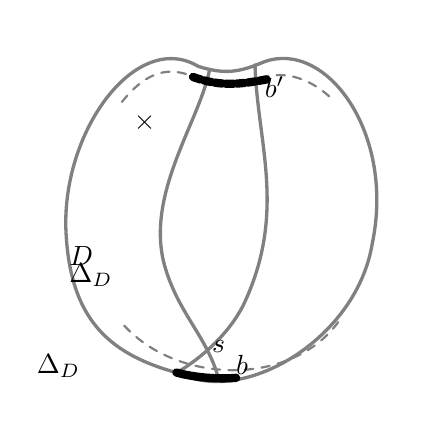
\begin{tikzpicture}[x=.96cm,y=.96cm,line cap=round,line join=round]
\draw[very thick,gray] (-.36,2.04) .. controls (-1.18,2.53) and (-2.18,1.18) .. (-2.11,-.16) .. controls (-2.05,-1.35) and (-1.5,-1.79) .. (-.58,-2.03) .. controls (.25,-2.43) and (1.73,-1.57) .. (1.94,-.31) .. controls (2.25,1.16) and (1.33,2.4) .. (.51,2.10) .. controls (.18,1.96) and (-.01,1.93) .. (-.36,2.04);
\draw[very thick,gray] (-.21,2) .. controls (-.34,1.32) and (-1.06,.36) .. (-.81,-.58) .. controls (-.64,-1.2) and (-.27,-1.51) .. (-.11,-2.03);
\draw[very thick,gray] (.39,2.06) .. controls (.42,1.02) and (.82,.1) .. (.23,-1.13) .. controls (-.01,-1.59) and (-.44,-1.89) .. (-.64,-2.01);
\draw[thick,dashed,gray] (-1.37,1.57) .. controls (-.91,2.15) and (-.57,1.94) .. (-.38,1.9);
\draw[thick,dashed,gray] (.46,1.89) .. controls (.82,1.99) and (1.14,1.87) .. (1.43,1.59);
\draw[thick,dashed,gray] (-1.34,-1.39) .. controls (-.61,-2.18) and (.89,-2.19) .. (1.50,-1.33);
\draw[line width=3pt,densely dotted] (-.43,1.9) .. controls (-.05,1.76) and (.23,1.81) .. (.56,1.87);
\draw[line width=3pt] (-.65,-2.01) .. controls (-.4,-2.08) and (-.08,-2.1) .. (.14,-2.08);
\node at (-1.07,1.29) {$\times$};\node at (.65,1.77) {$b'$};\node at (.22,-1.91) {$b$};\node at (-.09,-1.66) {$s$};
\node at (-1.91,-.47) {$D$};\node at (-1.78,-.72) {$\deleted{\unsure{\Delta_D}}$};\node at (-2.21,-1.92) {$\Delta_D$};
\end{tikzpicture}}

% @ L1–6 under drawings
huit façons ``standard'' de vriller $\Delta_D$ à $\Delta_{D'}$ suiv.$^{\mathrm t}$ \deleted{la} \deleted{une} isom. \unsure{(orienté)|(orient.)|(combinatoire)} d'un des deux arcs de transition \inserted{$a,a'$} sur $\Delta_{D'}$, avec l'un des deux arcs privilégiés $b$ (de transition) et $b'$ (son antipodique) sur $\Delta_D$, deux choix pour chaque choix d'un couple dans $\{a,a'\}\times\{b,b'\}$.

% @ L6–12 to R7
Donc huit façons à priori de construire une surface \inserted{cellulaire} ayant pour graphe $\Gamma_{\underline\Sigma}=\Gamma$, mais (sauf pour les \unsure{plongements|polygones} d'\unsure{un complexe|une courbe|un couloir} rouge, \unsure{différent|différents}) il n'y a que quatre cas différents de surfaces, car ce qu'on obtient par un choix $(\alpha,\beta,\unsure{\varphi|\sigma|\rho})$\inserted{iso. de recollt} et $(\alpha',\beta',\sigma')$ (où $\alpha',\beta',\sigma'$ déduits en composant avec les antipodismes) sont can. isom. (ils correspondent à la \ensuremath{=} circularisation de $\Gamma$, et les $\mathord{=}$ \unsure{réflexions|morphismes|multiplicateurs} de transition pour les or. loc. correspond. de ).

% @ R8–20
On peut en supposer, quitte à composer avec les antipodismes de part et d'autre, que $\beta=b$ -- ce qui revient à faire un choix où le sommet $s$ apparaît \deleted{\unsure{sur}} au voisinage de l'arc de transition choisi, sur la surface \unsure{vrillée|recollée} (au lieu qu'il soit rejeté aux antipodes, ce qui a l'air un peu idiot !)

% @ R, last two lines
\deleted{Pour les quatre choix (en fait, les huit)} qui
